\begin{question}
\noindent A space agency stores a satellite instrument inside a cuboid-shaped protective casing $ABCDEFGH$, as shown in the diagram.

\noindent The casing has length $AB = 12$ cm, width $BC = 5$ cm, and height $CG = 9$ cm.

\noindent During transport, the instrument must be packed with a rigid support rod placed along the diagonal $AG$, from one bottom corner to the opposite top corner of the casing.

\begin{center}
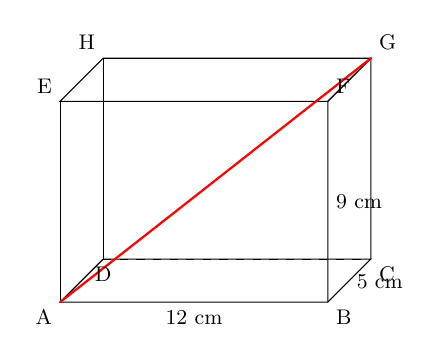
\begin{tikzpicture}[scale=0.85, transform shape]
    % Define the points of the cuboid (length 12, width 5, height 9)
    \coordinate (A) at (0,0,0);
    \coordinate (B) at (4,0,0);
    \coordinate (C) at (4,0,-1.67);
    \coordinate (D) at (0,0,-1.67);
    \coordinate (E) at (0,3,0);
    \coordinate (F) at (4,3,0);
    \coordinate (G) at (4,3,-1.67);
    \coordinate (H) at (0,3,-1.67);

    % Draw the visible edges of the cuboid
    \draw (A) -- (B) -- (C) -- (D) -- cycle; % bottom face
    \draw (B) -- (F) -- (G) -- (C); % right face
    \draw (E) -- (F) -- (G) -- (H) -- cycle; % top face
    \draw (A) -- (E);
    \draw (D) -- (H);

    % Draw the hidden edges
    \draw[dashed] (D) -- (C);

    % Diagonal AG
    \draw[thick, red] (A) -- (G);

    % Place the labels with smaller font size
    \node at (A) [below left, font=\small] {A};
    \node at (B) [below right, font=\small] {B};
    \node at (C) [below right, font=\small] {C};
    \node at (D) [below, font=\small] {D};
    \node at (E) [above left, font=\small] {E};
    \node at (F) [above right, font=\small] {F};
    \node at (G) [above right, font=\small] {G};
    \node at (H) [above left, font=\small] {H};

    \node at (2,0,0) [below, font=\small] {$12$ cm};
    \node at (4,0,-0.8) [right, font=\small] {$5$ cm};
    \node at (4,1.5,0) [right, font=\small] {$9$ cm};
\end{tikzpicture}
\end{center}

\noindent Calculate the length of the diagonal $AG$.

\noindent Give your answer correct to 3 significant figures.

\vspace{5cm}

\begin{flushright}
\answerunit{cm}{5}
\end{flushright}
\end{question}
